\documentclass[preview,border=3pt,convert={outext=.png}]{standalone}
\usepackage[left=1in,right=1in,top=1in,bottom=1in]{geometry} %set the page margins
\usepackage{tikz}
\usepackage{graphicx} % command that inserts common packages. This is required for inserting images.
\usepackage{xcolor}
\usepackage{amsmath,amsfonts,amsthm} %packages for math symbols



\begin{document}
% \bigg{\begin{equation}
%     B_i
% \end{equation}}
% \nopagecolor
\nopagecolor
% \verb|\nopagecolor|

% \mbox{\Huge $B_i$}

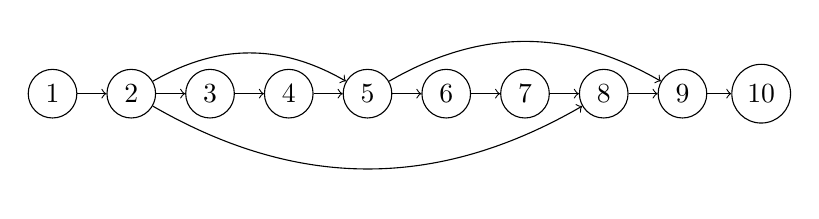
\begin{tikzpicture}[
  ->,
  node distance=1cm,
  every node/.style={circle, draw, minimum size=3mm}
]

\node (n1)  {1};
\node (n2)  [right of=n1] {2};
\node (n3)  [right of=n2] {3};
\node (n4)  [right of=n3] {4};
\node (n5)  [right of=n4] {5};

\node (n6)  [right of=n5] {6};
\node (n7)  [right of=n6] {7};
\node (n8)  [right of=n7] {8};
\node (n9)  [right of=n8] {9};
\node (n10) [right of=n9] {10};

\draw (n1)  -- (n2);
\draw (n2)  -- (n3);
\draw (n3)  -- (n4);
\draw (n4)  -- (n5);

% \draw (n1)  -- (n6);
\draw (n5)  -- (n6);
\draw (n5) edge[bend left] (n9);
% \draw (n3) edge[bend left] (n6);
\draw (n2) edge[bend left] (n5);
\draw (n2) edge[bend right] (n8);

\draw (n6)  -- (n7);
\draw (n7)  -- (n8);
\draw (n8)  -- (n9);
\draw (n9)  -- (n10);

% \draw (n10) edge[bend left] (n1);

\end{tikzpicture}

\end{document}